\item Perhatikan grafik gaya ($F$) vs waktu ($t$) di bawah ini!\\
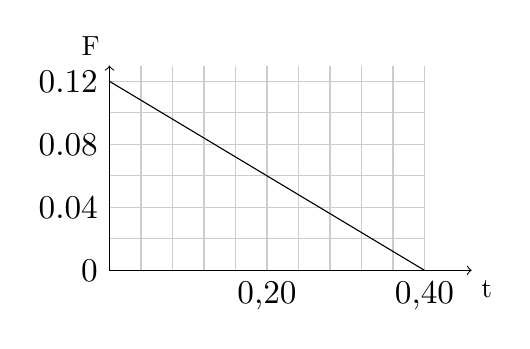
\begin{tikzpicture}[scale=0.2]

\draw [gray!40] (0,0) grid [step=2cm] (20,13);
\draw [<->](0,13)node [above left] {F}--(0,0)--(23,0)node [below right] {t};
\foreach \l / \y  in {0/0,0.04/4,0.08/8,0.12/12}
{ \node at (0,\y)[left,scale=1.2]{\l}; 
}
\node at (10,0) [below, scale=1.2] {0,20}; 
\node at (20,0) [below, scale=1.2] {0,40}; 

\draw(0,12) --(20,0);
\end{tikzpicture}
Besar impuls adalah . . . . \\
\pilgan{
\item [\lingkaran{A.}]0,024 Ns
\item 0,011 Ns
\item 0,005 Ns
\item 0.0101 Ns
\item 0,204 Ns
}
\item Gambar di bawah ini menunjukkan resultan gaya yang bekerja pada suatu benda terhadap waktu. Besar perubahan momentum benda setelah 15 s adalah . . . .\\
\begin{tikzpicture}[scale=0.3]
\draw [<->](0,12)node [above left] {F}--(0,0)--(17,0)node [below right] {t};
\foreach \x  in {5,10,15}
{ \node at (\x,0)[below,scale=1.2]{\x}; 
} 
\draw(0,10) node [left,scale=1.2] {10}--(5,10)--(15,0);
\draw[dashed](5,10)--(5,0)--(10,0)--(10,5)--(0,5);
\node at (0,5) [left,scale=1.2] {5};
\end{tikzpicture}
\pilgan{
\item 50 Ns
\item [\lingkaran{B.}]100 Ns
\item 150 Ns
\item 200 Ns
\item 250 Ns
} 
